\begin{appendix}
    \section{Related Work}
\label{related}
Continual learning has been an active area of research in which many researchers have proposed techniques for mitigating catastrophic forgetting. The main idea behind these methods is to balance stability (retaining knowledge) and plasticity (learning new concepts) for deep learning models. Techniques broadly fall into three categories~\cite{de2021continual}: regularisation-based~\cite{kirkpatrick2017overcoming, li2017learning, shin2017continual, wu2019large}, replay-based~\cite{rebuffi2017icarl, chaudhry2018efficient, ostapenko2019learning, buzzega2020dark}, and parameter-isolation methods~\cite{rusu2016progressive, serra2018overcoming}. State-of-the-art performance often combines these approaches~\cite{mittal2021essentials}.

\subsection{Continual Self-supervised Learning}
However, many existing techniques rely heavily on labelled data, which is often unavailable.  Continual self-supervised learning (CSSL) approaches leverage self-supervised learning to enable continual learning under limited supervision. Initial efforts focused narrowly on self-supervised pre-training combined with supervised continual learning~\cite{gallardo2021self, caccia2022special} or extending contrastive learning frameworks~\cite{cha2021co2l, madaan2021rethinking}. However, these techniques are often designed to work with specific self-supervised learning frameworks. The latest continual self-supervised learning frameworks proposed in existing literature~\cite{de2021continual, fini2022self} have begun investigating more overarching and flexible frameworks, where the model learns continually from a stream of unlabelled data. The work by \cite{tang2023practical} proposed a unified semi-supervised framework with continual fine-tuning, introducing mechanisms for knowledge distillation and new task learning in both representation and classification. These demonstrate progress towards practical solutions under realistic supervision assumptions, and we focus on these recent proposals which repurpose SSL methods for continual learning in this work.

\subsection{Human Activity Recognition}
Wearable-based human activity recognition is an important component in human-centric computing because of its ability to extract real-time information and context clues about user behaviours, which enables other computing applications \cite{choi2016understanding, jaimes2015corredor}. However, the utility of HAR systems has been limited by the scarcity of high-quality labelled data and the computational capabilities of wearable devices.

Since the adoption of deep learning models for HAR, researchers have looked at tackling catastrophic forgetting in HAR specifically \cite{jha2021continual, leite2022resource, schiemer2023online}, and they have demonstrated moderate success. Simultaneously, self-supervised learning has recently gained popularity in the wearable-based HAR community, and many approaches from the general machine learning community, as well as customised methods, have been proposed to leverage unlabelled data to overcome the limitations of labelled data \cite{multi_self_har, tang2020exploring, haresamudram2020masked, tang2021selfhar, haresamudram2021contrastive}. However, we have yet to see efforts in leveraing self-supervised learning techniques for HAR in continual learning. This is an important step towards practical and generalisable user models. CSSL paves the way for realistic solutions to continually learn from combinations of labelled and unlabelled data.

\section{Transformation Functions}
\label{appx:trans}

\noindent\textbf{Random 3D rotation} applies a random rotation in the 3D space by picking a random axis in 3D and a rotational angle from uniform distributions. This is to simulate common pose changes in wearable devices.

\noindent\textbf{Random scaling} alters the size of samples within a window by multiplying them with a randomly chosen scalar. We apply this transformation since a model that can handle these scaled signals creates better representations because it learns to be unaffected by changes in amplitude and offset.

\noindent\textbf{Time warping} locally stretches or warps the time series data, smoothly distorting the time intervals between sensor readings.
\section{Evaluation setup}
\label{appx:setup}
{
\subsection{Model Architecture}
In this work, we adopted a lightweight HAR model, TPN \cite{multi_self_har}, to replace the vision-based model.

\subsection{Evaluation Metrics}
For the evaluation metrics, we are adopting the same framework as introduced in Kaizen \cite{tang2023practical}: \textbf{Final Accuracy (FA)}, \textbf{Continual Accuracy (CA)}, \textbf{Forgetting (F)}, and \textbf{Forward Transfer (FT)} as metrics. This set of values can better reflect the performance of continual learning methods in different use cases.

\subsection{Self-supervised Learning Frameworks}
In this work we selected a contrastive-based method MoCoV2+~\cite{chen2020improved, he2020momentum}, and an asymmetric-model-based method
BYOL~\cite{grill2020bootstrap} as the self-supervised learning method for continual learning. These two methods have been shown to be well-performing in continual self-supervised learning settings~\cite{fini2022self, tang2023practical}, and our goal is to investigate whether different CSSL methods demonstrate different performance characteristics when using different SSL methods as the knowledge retention mechanism.

\subsection{Dataset}
We performed our evaluation using the WISDM2019 (WISDM Smartphone and Smartwatch Activity and Biometrics Dataset) \cite{weiss2019wisdm}, which is an activity recognition dataset collected by the WISDM (Wireless Sensor Data Mining) Lab in the Department of Computer and Information Science of Fordham Unversity. The dataset contains raw accelerometer and gyroscope data from a smartwatch (LG G Watch) and a smartphone (Google Nexus 5/5x or Samsung Galaxy S5) worn by 51 subjects, who performed 18 different activities for 3 minutes each. The smartphone is placed inside the participant's pocket, while the smartwatch is worn at the dominant hand. The data was collected at a sampling rate of 20Hz for the following activities: Walking, Jogging, Stairs, Sitting, Standing, Typing, Brushing Teeth, Eating Soup, Eating Chips, Eating Pasta, Drinking from Cup, Eating Sandwich, Kicking (Soccer Ball), Playing Catch with Tennis Ball, Dribbling (Basketball), Writing, Clapping, and Folding Clothes. The accelerometer data from the smartwatch was used in this study, and we selected this dataset for evaluation because it has a relatively high number of activities in HAR, which makes it suitable for continual learning evaluation.

The raw sensor data underwent minimal pre-processing. First, z-normalization was applied using the training data's mean and standard deviation for each sensor channel. Next, the data was segmented into \(384 \times 3\) sliding windows, representing 384 timestamps and 3 triaxial accelerometer channels. Consecutive windows do not overlap. 20-25\% of user data was held out unseen as the test set to evaluate model generalisability. 

The 18 classes of activities are randomly and evenly split into 6 tasks of 3 classes each with no overlap as follows: task 1 - \{Folding Clothes, Stairs, Walking\}, 
task 2 - \{Sitting, Drinking from Cup, Eating Chips\}, 
task 3 - \{Standing, Eating Sandwich, Clapping\}, 
task 4 - \{Brushing Teeth, Jogging, Eating Pasta\},
task 5 - \{Eating Soup, writing, Typing\}, and
task 6 - \{Playing Catch with Tennis Ball, Kicking (Soccer Ball), Dribbling (Basketball)\}. This follows the conventional setup of class-incremental learning, and how different (potentially qualitative) splitting of the classes affects model performance is left as future work.

\subsection{Baselines}
\label{subsection:baselines}
We followed the evaluation setup as proposed in \cite{tang2023practical}, in which we compare the performance of Kaizen, CaSSLe, as well as a \emph{No distill} baseline that fine-tunes the full model on new tasks with no explicit catastrophic forgetting mitigation. As CaSSLe and \emph{No distill} baselines are self-supervised learning methods without incorporating a classifier, the classifiers are trained separately after the feature extractor is trained, with data replay enabled.
}
\end{appendix}

\section{Additional Visualisations}
\label{subsection:additional_results}
\begin{figure}
    \centering
    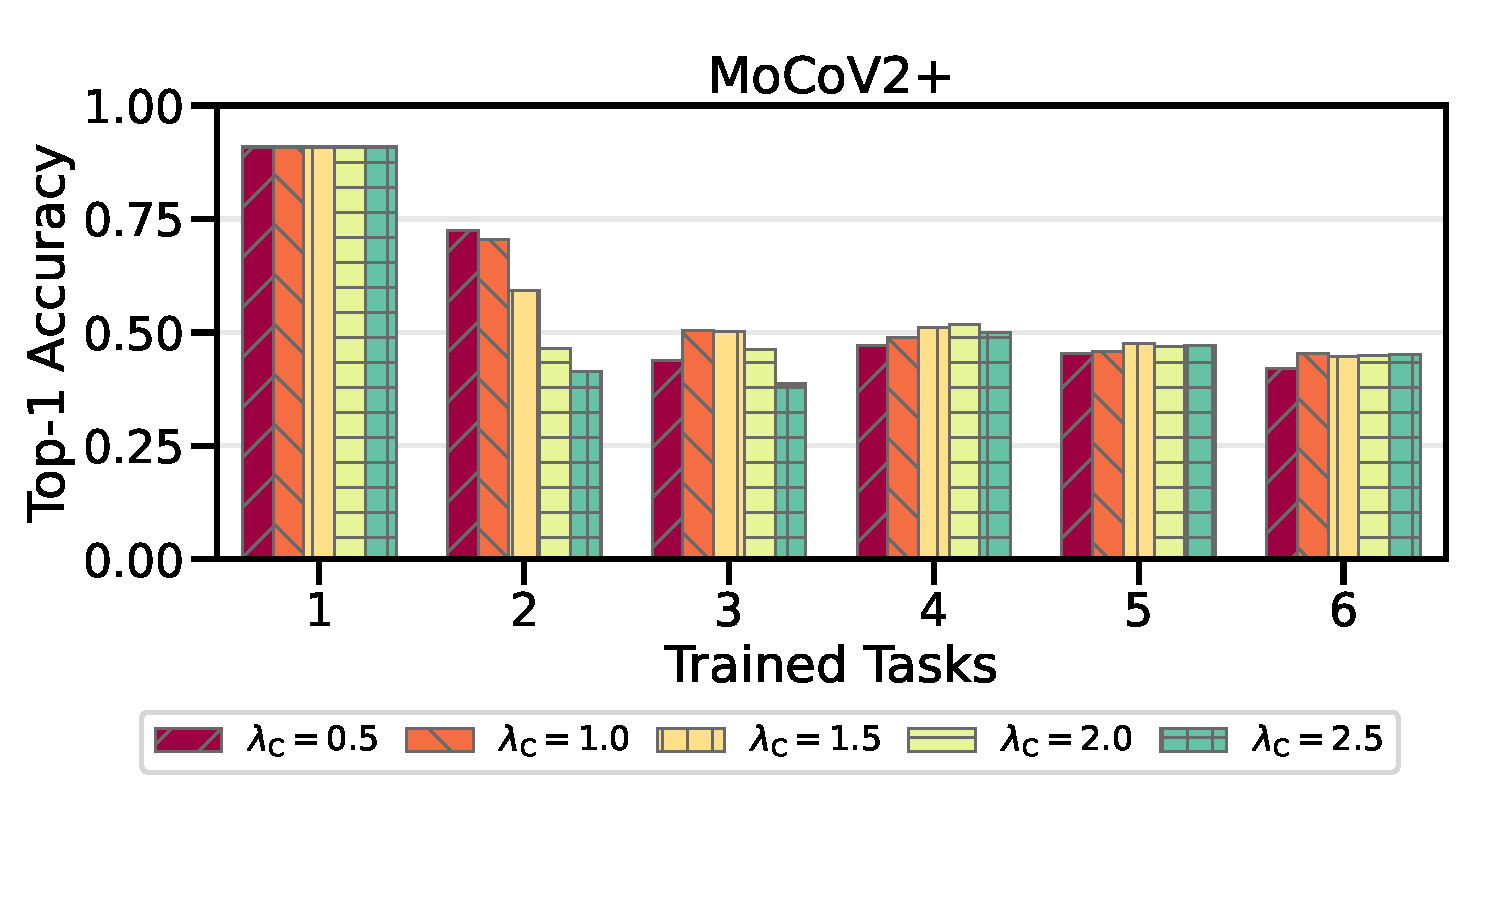
\includegraphics[width=0.8 \linewidth ]{figures_new/Part_2/F3-WISDM2019-MoCoV2+-6Tasks-v2.pdf}
    % \vspace{-0.3in}
    \caption{Performance after training on different tasks with varying constant importance coefficients.}
\label{fig:kaizen_performance_across_time_constant_lamb}
\end{figure}


\begin{figure}
    \centering
    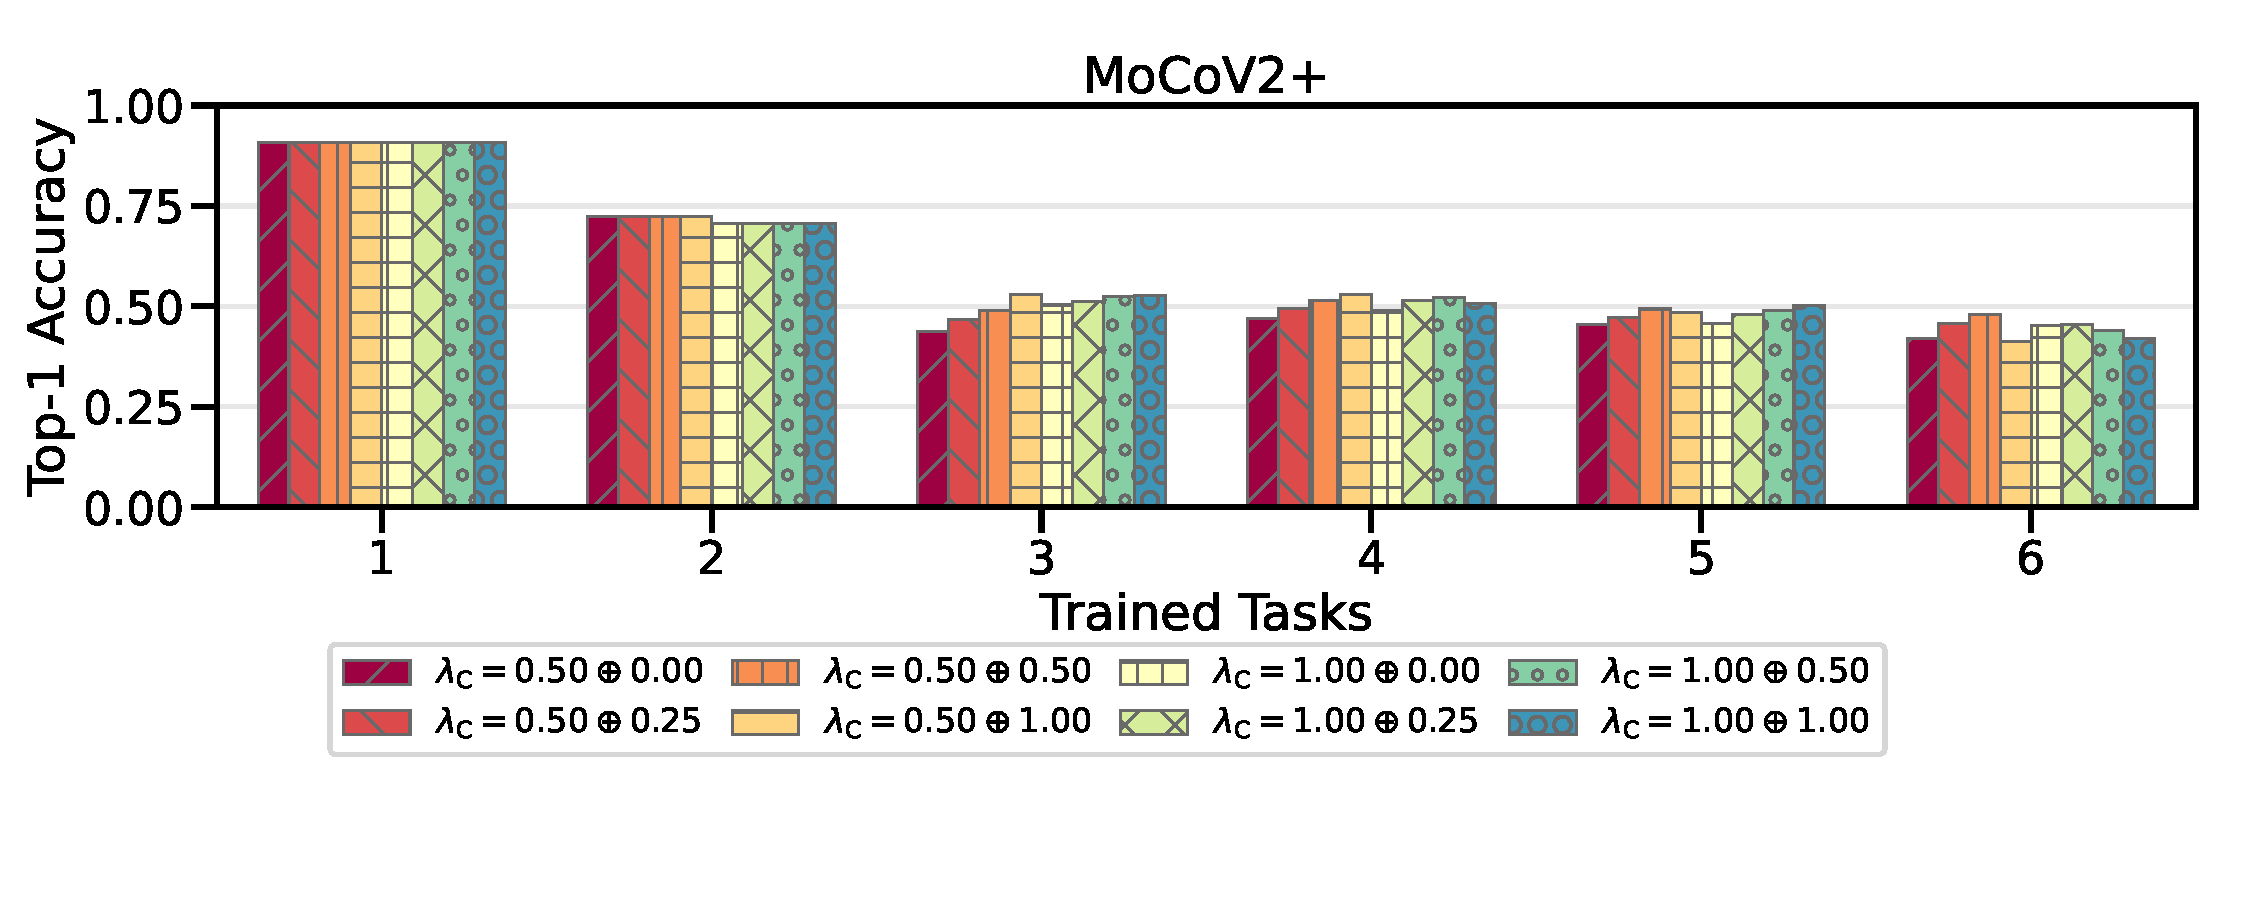
\includegraphics[width=0.99 \linewidth ]{figures_new/Part_3/F3-WISDM2019-MoCoV2+-6Tasks-v2.pdf}
    % \vspace{-0.3in}
    \caption{Performance after training on different tasks with varying progressive importance coefficients.}
\label{fig:kaizen_performance_across_time_progressive_lamb}
\end{figure}

Fig.~\ref{fig:kaizen_performance_across_time_constant_lamb} and \ref{fig:kaizen_performance_across_time_progressive_lamb} illustrate the aggregated performance of models trained with Kaizen after each task with different importance coefficients.
